
\section{Основная часть}

    \subsection{Определение модели}

        Модель Hassell имеет следующую математическая запись:

        \[x_{t+1} = \frac{\alpha x_t^2}{(\beta + x_t)^6}\]

        где \(x_i\) --- количество особей в поколении с номером i. Параметр \(\alpha\) определяет скорость роста популяции, а параметр \(\beta\) определяет несущую способность окружающей среды.
    
    \subsection{Частный случай}
    
        Зафиксируем параметр \(\alpha = 1\). Параметр \(\beta\) изменяется в диапазоне \([0; 0.6]\). Также запишем уравнение в таком виде:

        \[x = \frac{\alpha x^2}{(\beta + x)^6}\]
    
        \[1 = \frac{\alpha x}{(\beta + x)^6}\]

        \[\alpha x = (\beta + x)^6\]

        Теперь можно построить графики функций \(y = \alpha x\) и \(y = (\beta + x)^6\). В зависимости от значений параметра \(\beta\) уравнение может иметь ноль, одну или две общие точки. На рисунках (\ref{mainIntersect}), (\ref{mainTouch}), (\ref{mainOver}) можно увидеть все возможные варианты.
        
        \begin{figure}
            \centering
            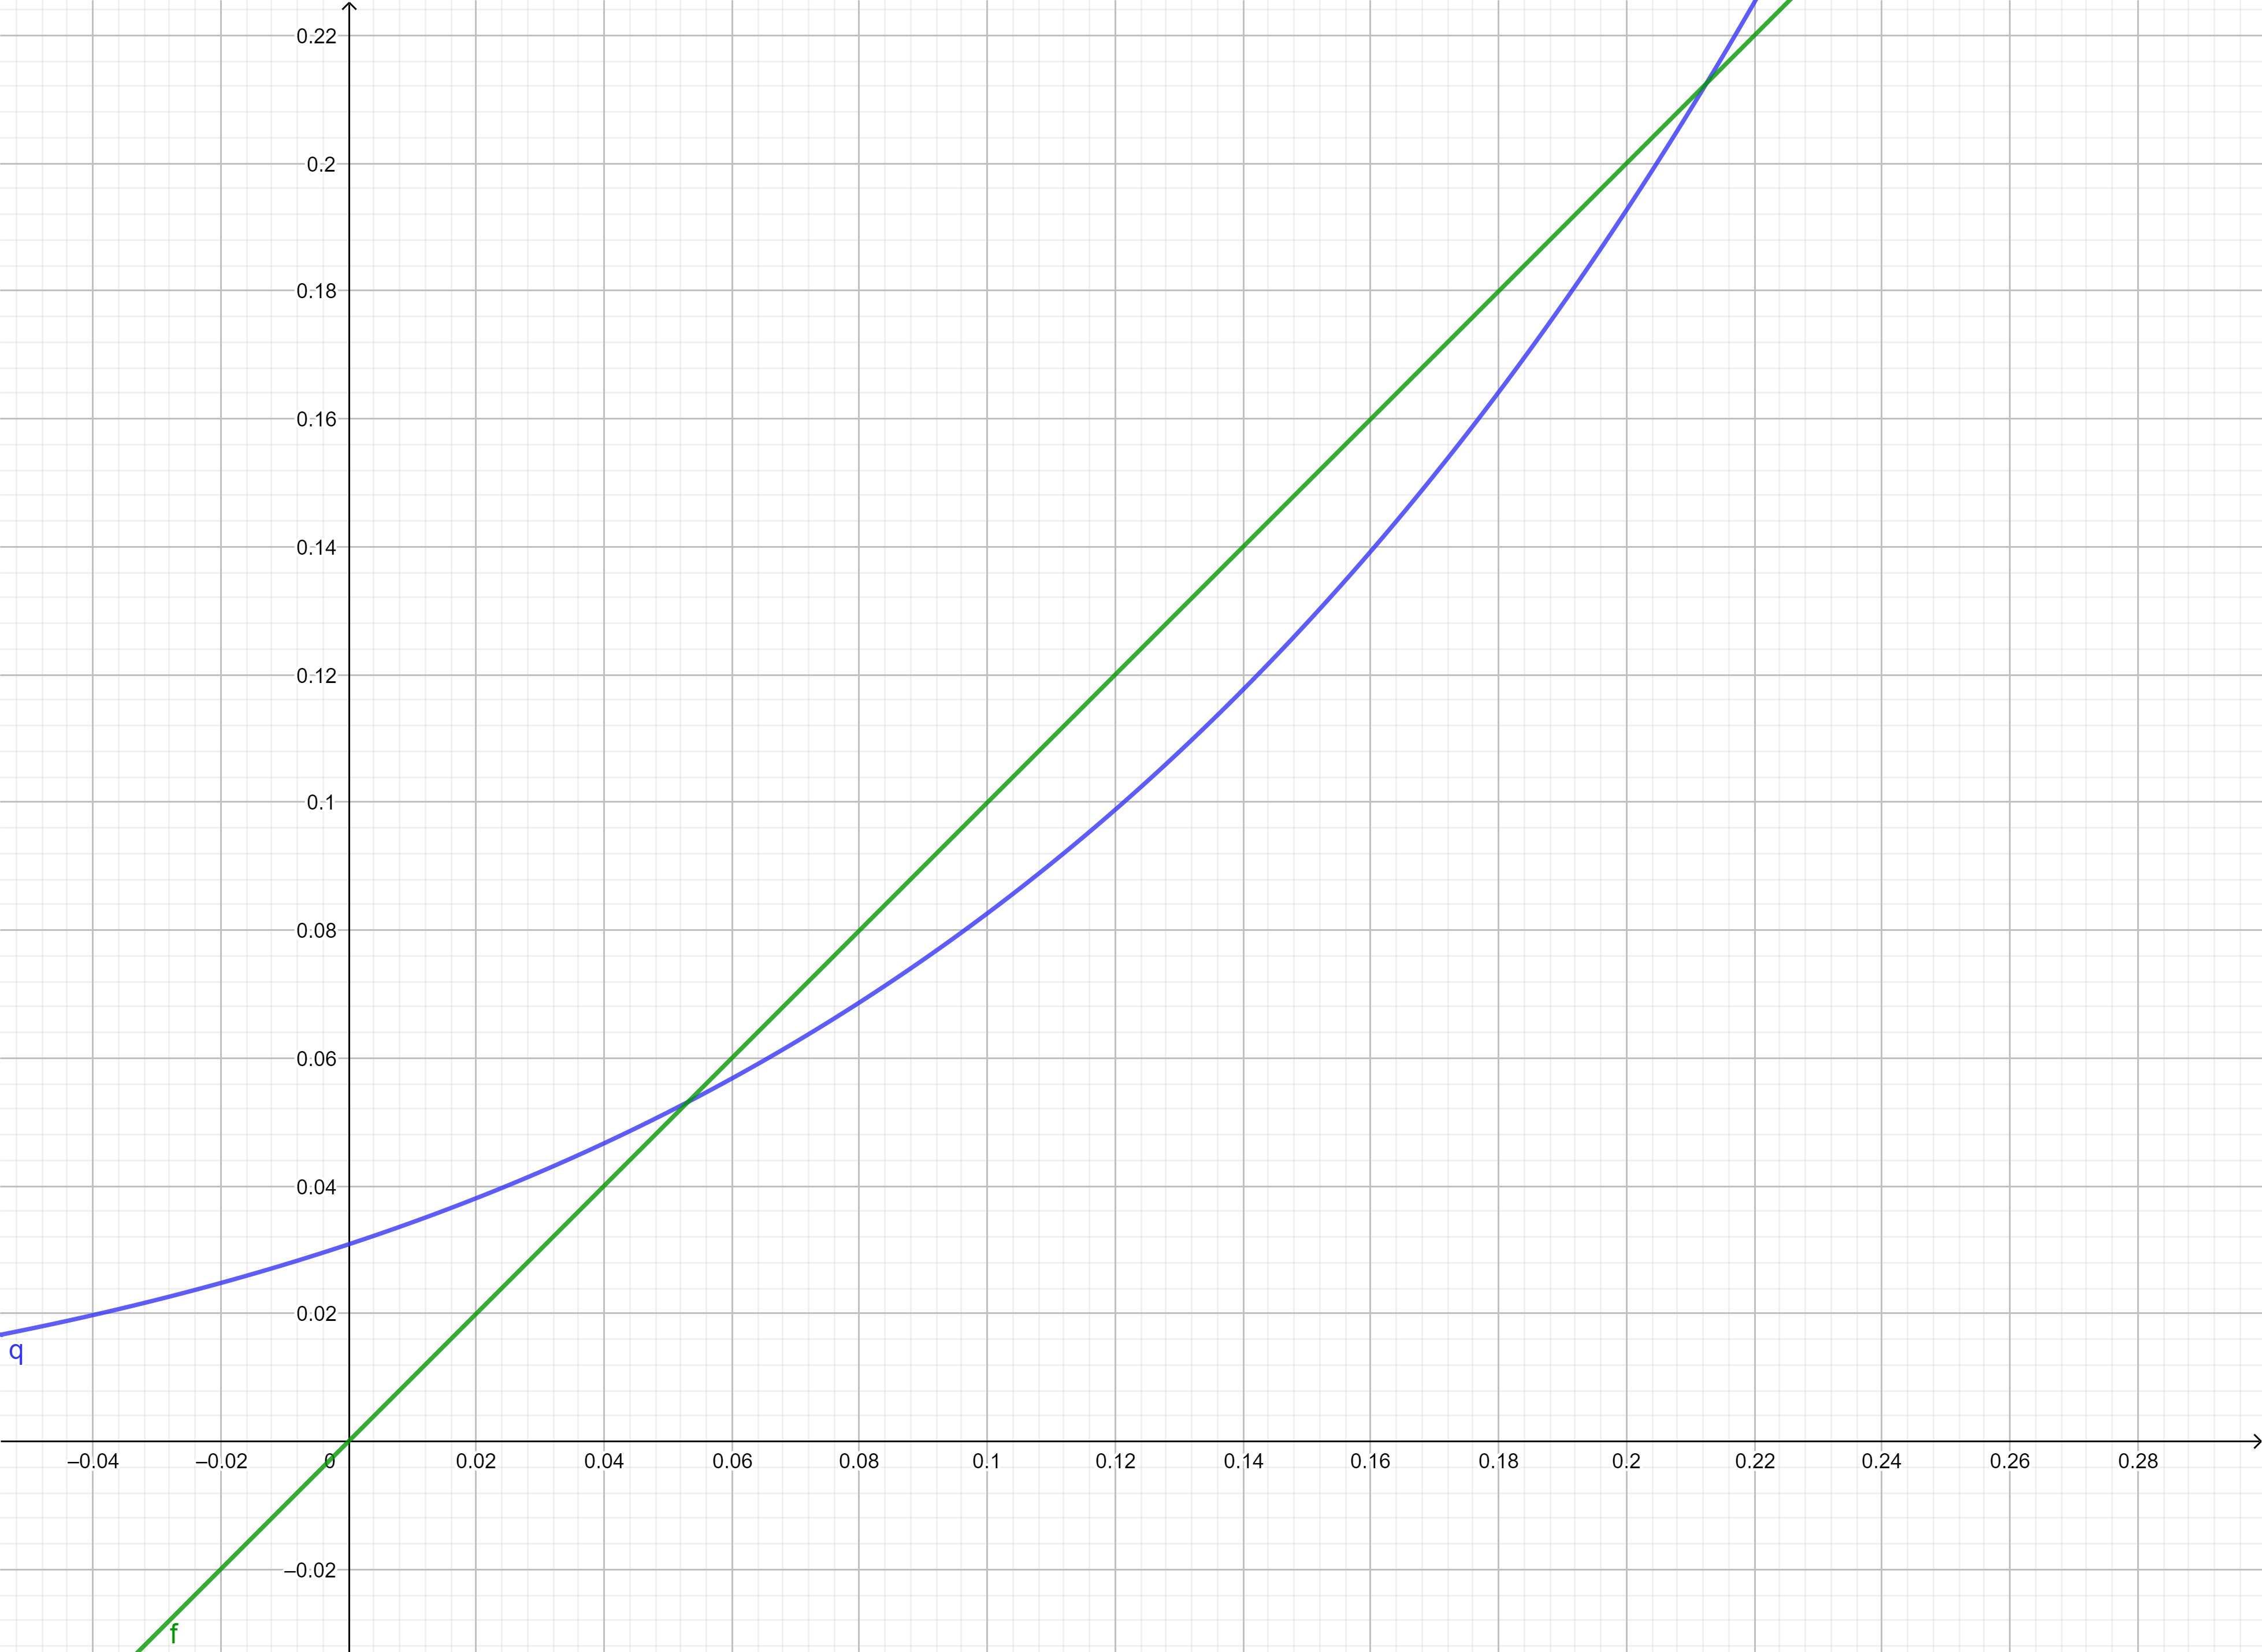
\includegraphics[width=\textwidth]{images/main_intersect.jpg}

            \captionsetup{justification=centering}
            \caption{\(\beta < 0.582355932\)}
            \label{mainIntersect}
        \end{figure}

        \begin{figure}
            \centering
            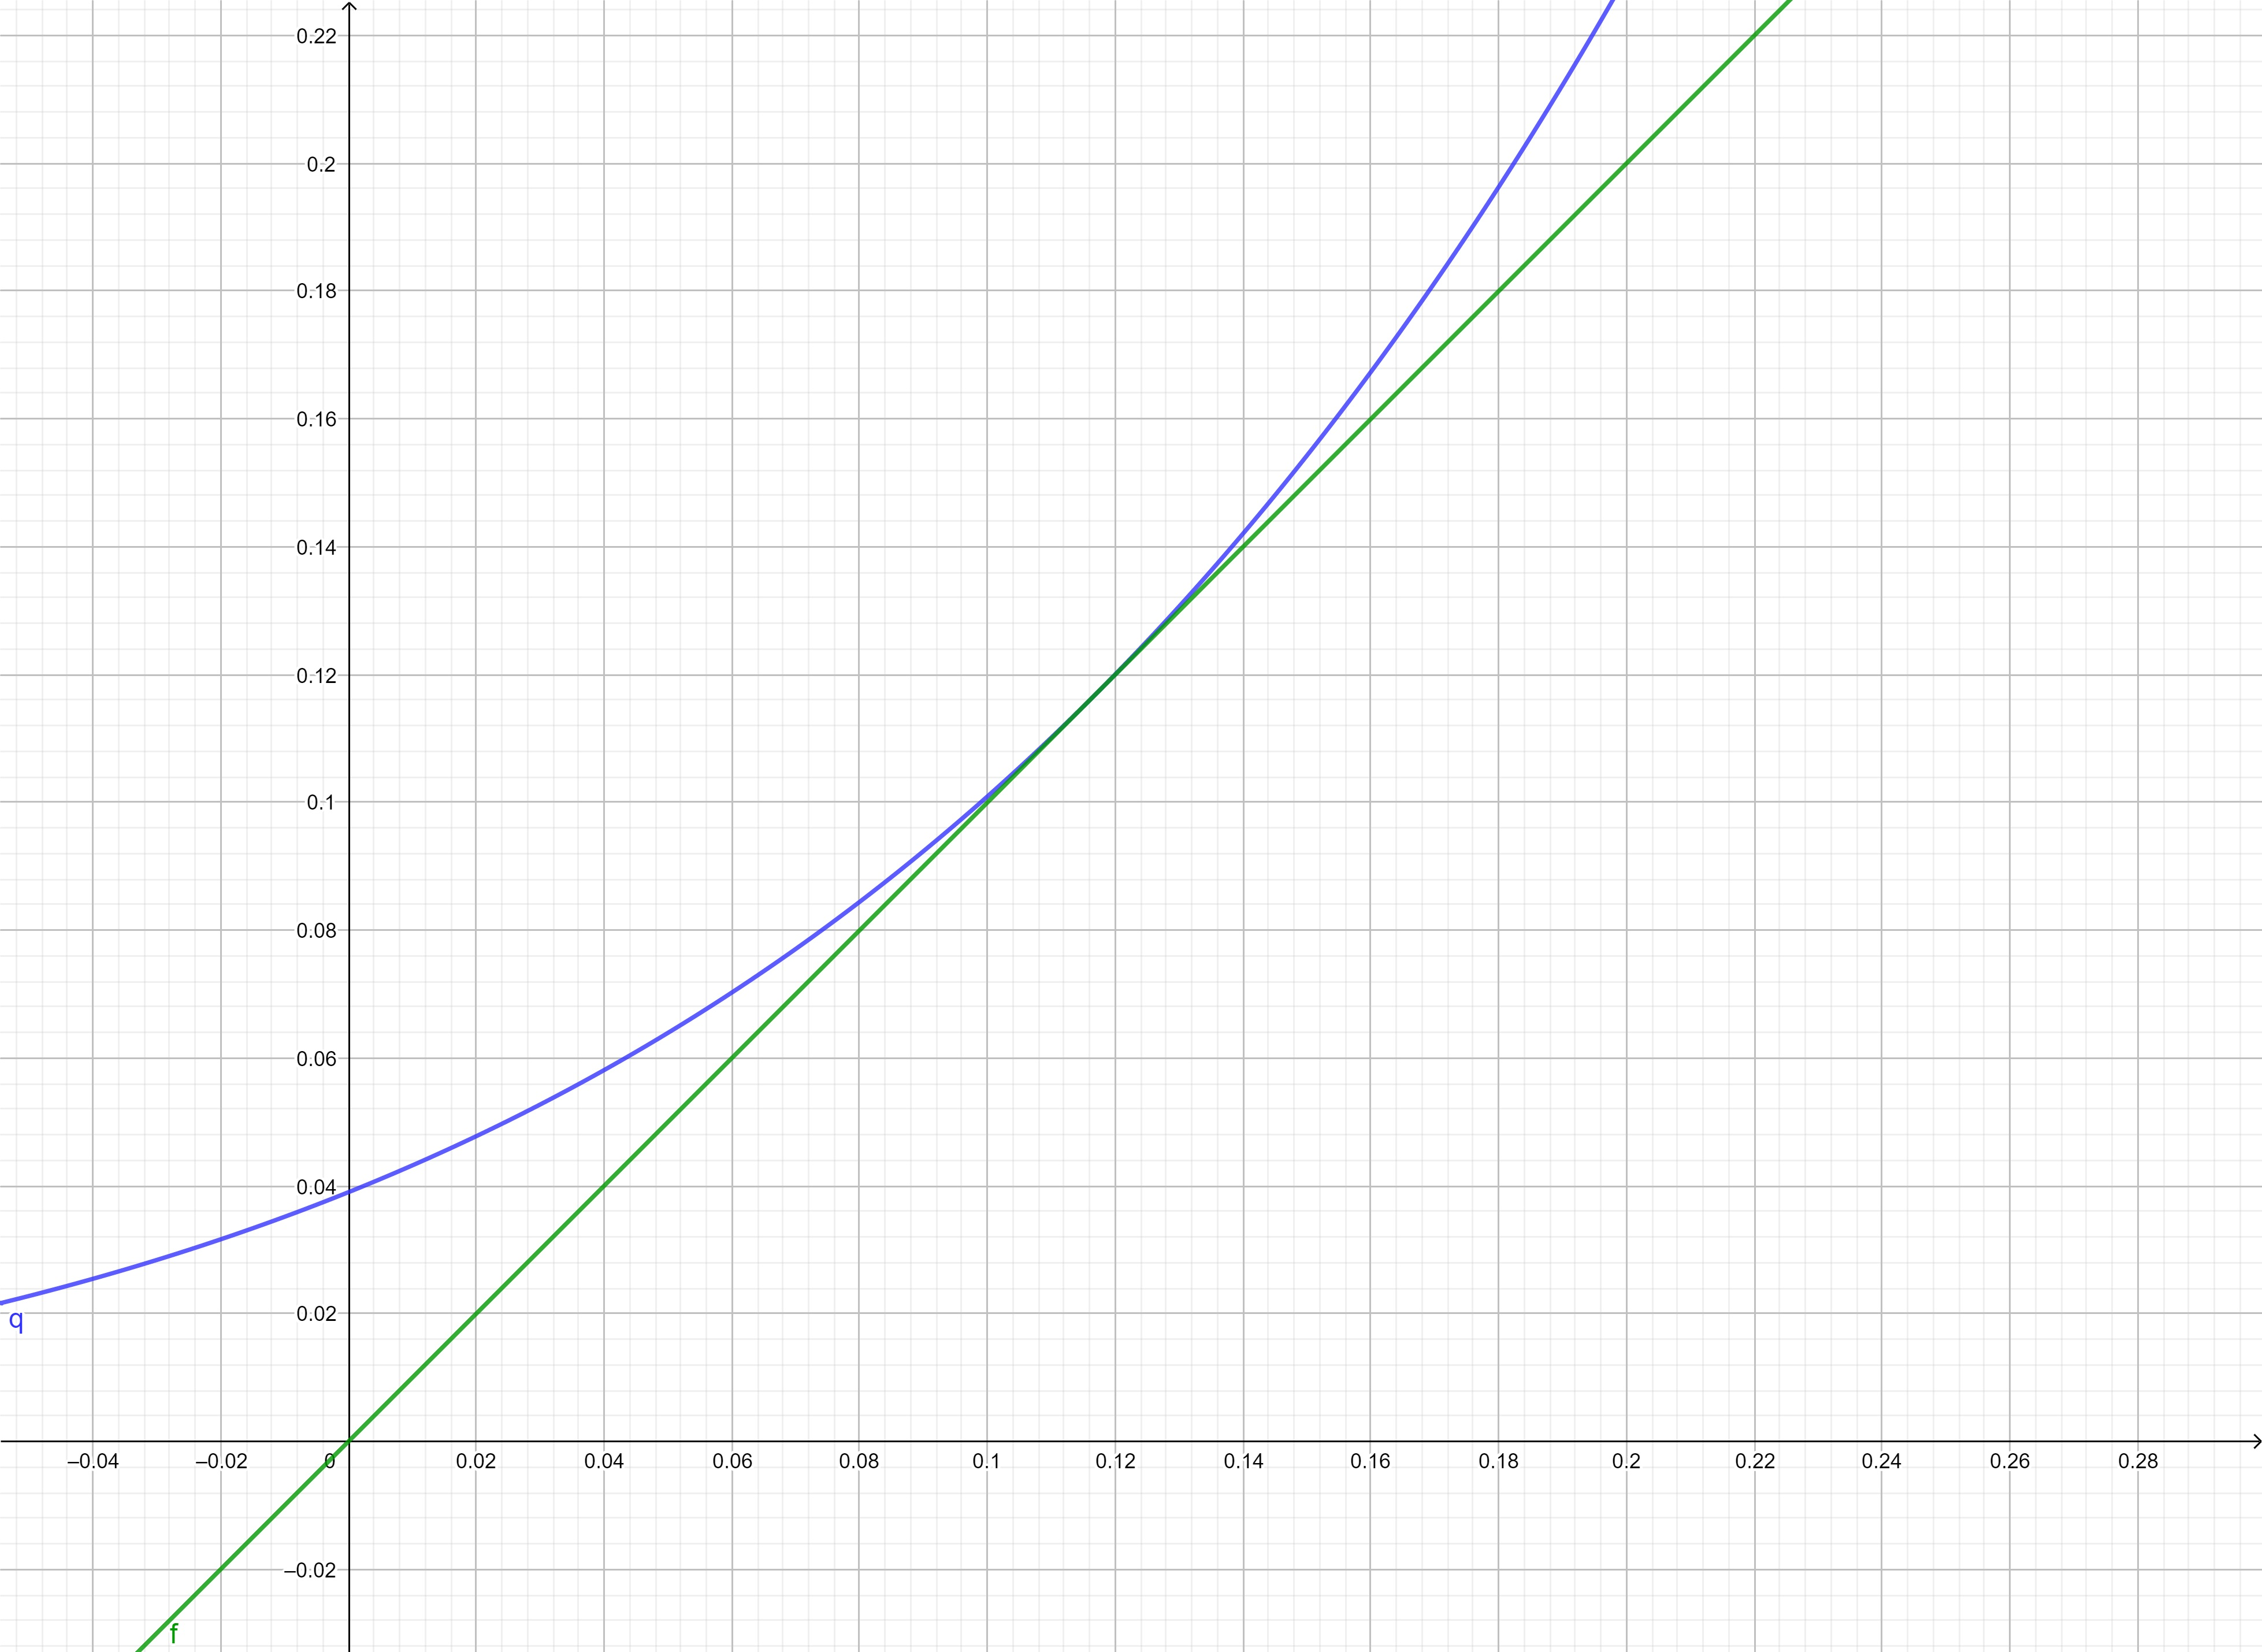
\includegraphics[width=\textwidth]{images/main_touch.jpg}

            \captionsetup{justification=centering}
            \caption{\(\beta \approx 0.582355932\)}
            \label{mainTouch}
        \end{figure}

        \begin{figure}
            \centering
            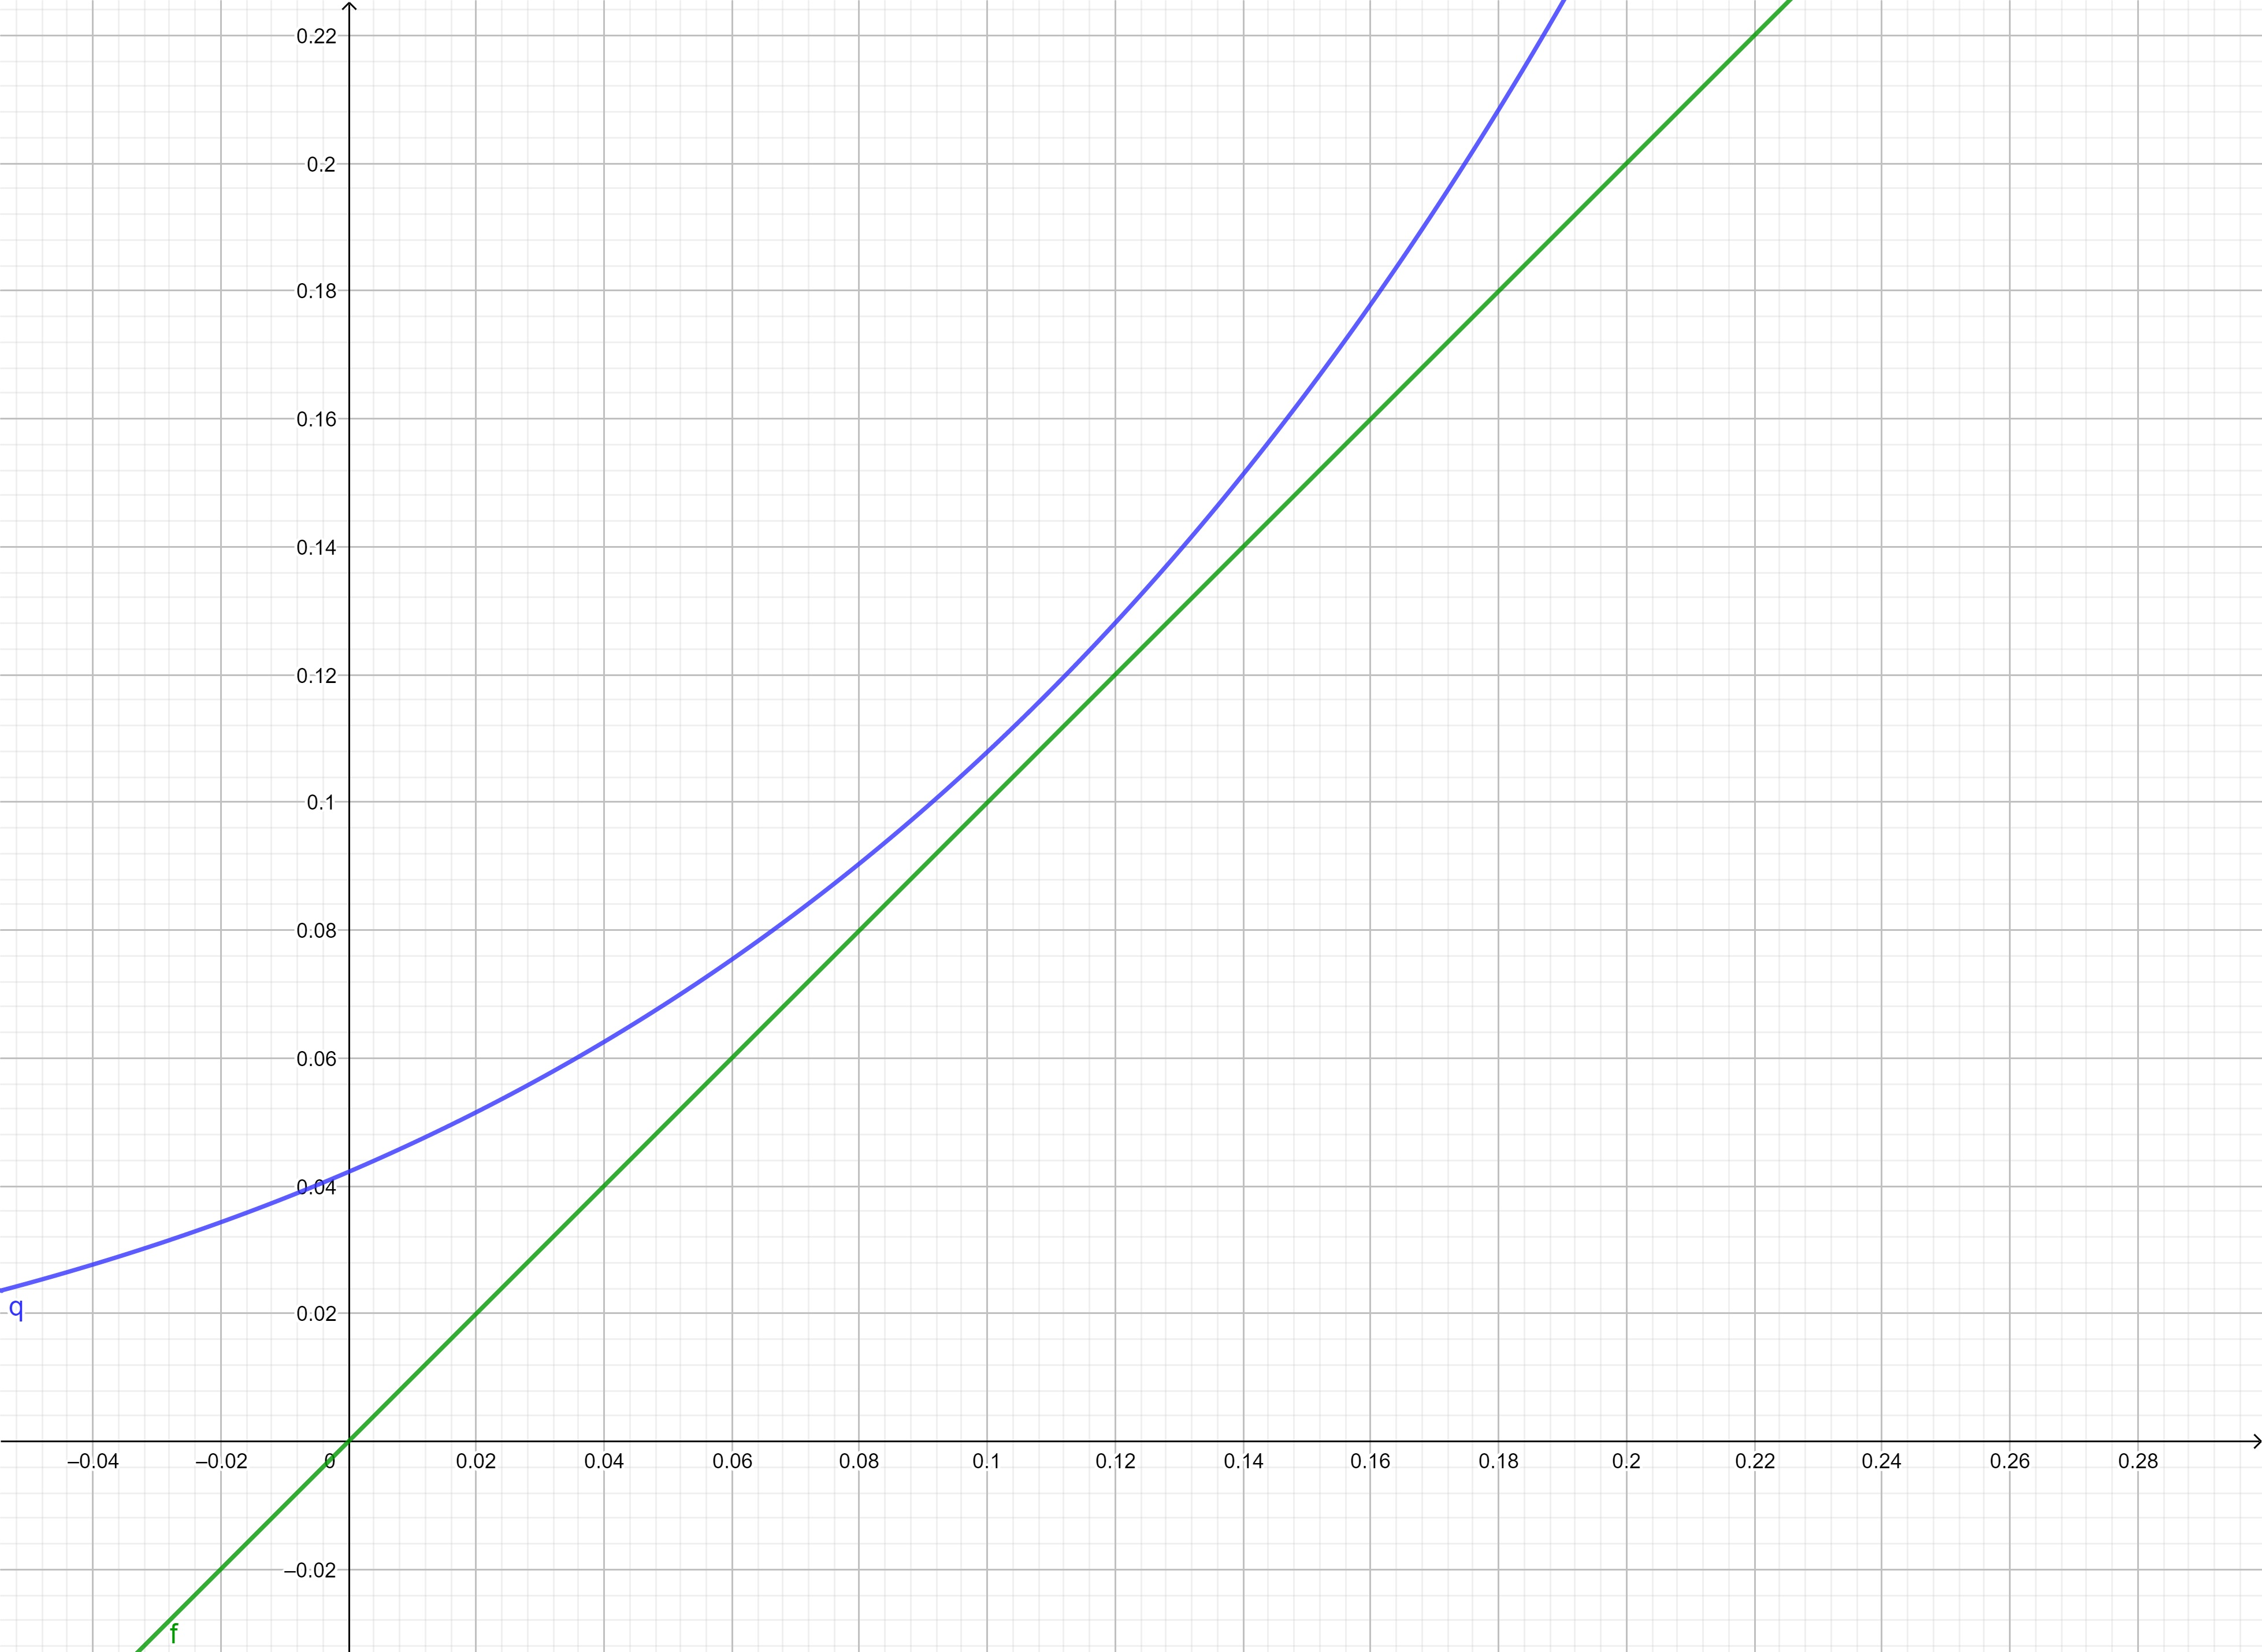
\includegraphics[width=\textwidth]{images/main_over.jpg}

            \captionsetup{justification=centering}
            \caption{\(\beta > 0.582355932\)}
            \label{mainOver}
        \end{figure}

        Аналитически это уравнение не решается. Для нахождения корней я буду использовать метод Ньютона. В зависимости от конкретных значений параметра \(\beta\) данное уравнение может иметь от одного до трех корней.

    \subsection{Временные ряды}

        Для анализа системы можно использовать временные ряды. Временной ряд позволяет наглядно показать как с течением времени изменяется численность популяции.

        Например, на графике (\ref{timeSeriesX=0.02b=0.55}) мы видим, что при начальных значениях \(x = 0.02\) и \(\beta = 0.55\) временной ряд сходятся к нулю. В биологическом смысле это означает, что популяция с теченеим времени вымирает.
    
        \begin{figure}[h!]
            \centering
            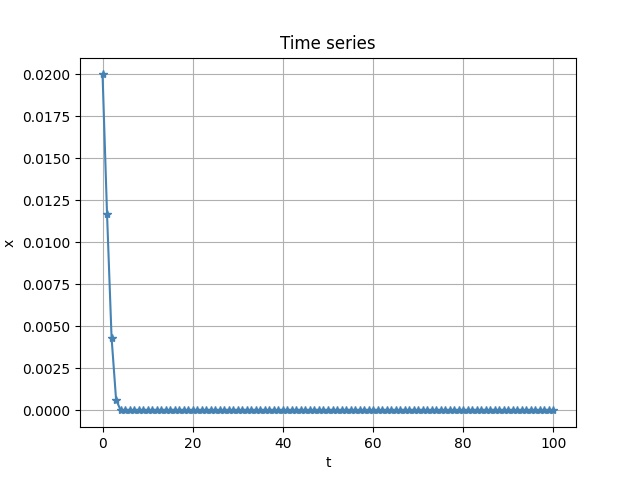
\includegraphics[width=0.8\textwidth]{Time_series._x_0.02_b_0.55.jpeg}

            \captionsetup{justification=centering}
            \caption{\(x_0 = 0.02; \beta = 0.55\)}
            \label{timeSeriesX=0.02b=0.55}
        \end{figure}

        На графике (\ref{timeSeriesX=0.05b=0.48}) видно, что при начальных условиях \(x = 0.05, \beta = 0.48\) популяция очень быстро растет до некоторого предела. После достижения данного предела начинается процесс стабилизации, т.е. значения стремятся к устойчивому равновесию \(x \approx 0.3656\). Это значит, что популяция с течением времени стабилизируется и перестанет расти или вымирать.

        Аналогичную ситуацию мы можем наблюдать на графике (\ref{timeSeriesX=0.05b=0.55}).
    
        \begin{figure}[h!]
            \centering
            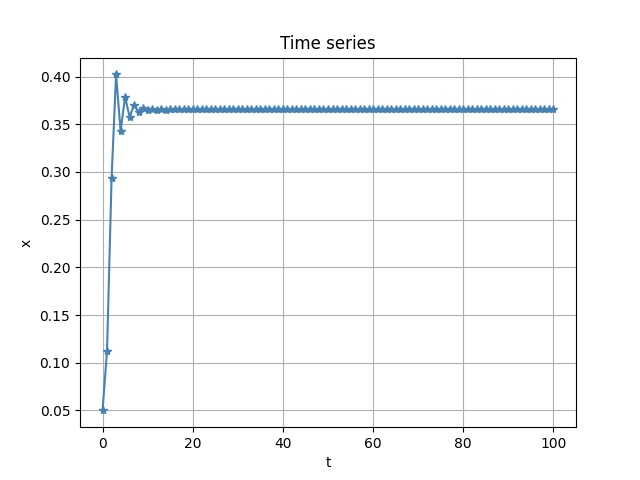
\includegraphics[width=0.8\textwidth]{Time_series._x_0.05_b_0.48.jpeg}

            \captionsetup{justification=centering}
            \caption{\(x_0 = 0.05; \beta = 0.48\)}
            \label{timeSeriesX=0.05b=0.48}
        \end{figure}
    
        \begin{figure}[h!]
            \centering
            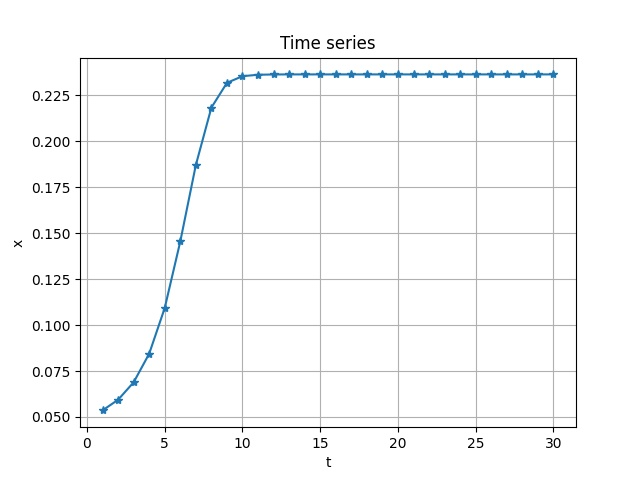
\includegraphics[width=0.8\textwidth]{Time_series._x_0.05_b_0.55.jpeg}

            \captionsetup{justification=centering}
            \caption{\(x_0 = 0.05; \beta = 0.55\)}
            \label{timeSeriesX=0.05b=0.55}
        \end{figure}

    \subsection{График бифуркации}

    \subsection{Лестница Ламери}

    \subsection{Показатели Ляпунова}

    \subsection{Недоделанная карта режимов}